
\begin{figure}[htbp]
\centering
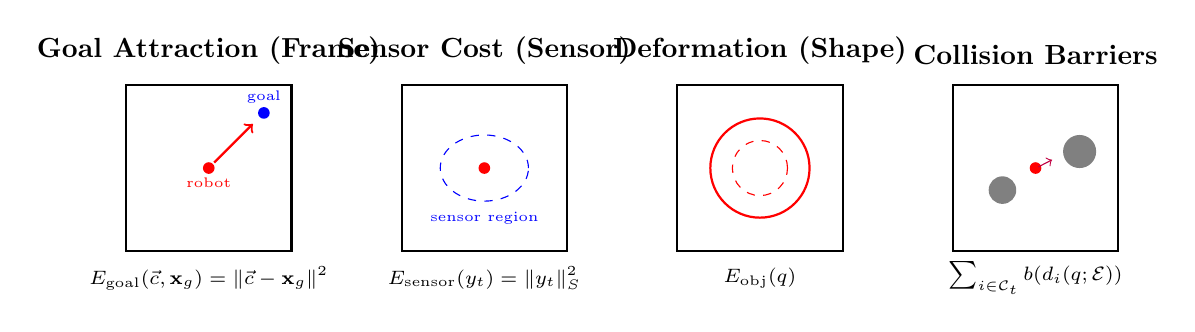
\begin{tikzpicture}[scale=0.7]

% Goal Attraction (Frame Policy)
\begin{scope}[shift={(-7.5,2)}]
    \draw[thick] (-1.5,-1.5) rectangle (1.5,1.5);
    \node[above] at (0,1.7) {\textbf{Goal Attraction (Frame)}};
    \fill[red] (0,0) circle (3pt) node[below] {\tiny robot};
    \fill[blue] (1,1) circle (3pt) node[above] {\tiny goal};
    \draw[->,thick,red] (0.1,0.1) -- (0.8,0.8);
    \node at (0,-2) {\scriptsize $E_{\mathrm{goal}}(\vec{c},\mathbf{x}_g) = \|\vec{c}-\mathbf{x}_g\|^2$};
\end{scope}

% Sensor Cost (Sensor Policy)
\begin{scope}[shift={(-2.5,2)}]
    \draw[thick] (-1.5,-1.5) rectangle (1.5,1.5);
    \node[above] at (0,1.7) {\textbf{Sensor Cost (Sensor)}};
    \fill[red] (0,0) circle (3pt);
    \draw[blue,dashed] (0,0) ellipse (0.8 and 0.6);
    \node[blue] at (0,-0.9) {\tiny sensor region};
    \node at (0,-2) {\scriptsize $E_{\mathrm{sensor}}(y_t)=\|y_t\|_{S}^2$};
\end{scope}

% Deformation (Shape Policy)
\begin{scope}[shift={(2.5,2)}]
    \draw[thick] (-1.5,-1.5) rectangle (1.5,1.5);
    \node[above] at (0,1.7) {\textbf{Deformation (Shape)}};
    \draw[red,thick] (0,0) circle (0.9);   % expanded radius
    \draw[red,dashed] (0,0) circle (0.5); % contracted radius
    \node at (0,-2) {\scriptsize $E_{\mathrm{obj}}(q)$};
\end{scope}

% Collision Barriers
\begin{scope}[shift={(7.5,2)}]
    \draw[thick] (-1.5,-1.5) rectangle (1.5,1.5);
    \node[above] at (0,1.7) {\textbf{Collision Barriers}};
    \fill[red] (0,0) circle (3pt);
    \fill[gray] (0.8,0.3) circle (0.3);
    \fill[gray] (-0.6,-0.4) circle (0.25);
    \draw[->,purple] (0.05,0.02) -- (0.3,0.15);
    \node at (0,-2) {\scriptsize $\sum_{i\in\mathcal{C}_t} b(d_i(q;\mathcal{E}))$};
\end{scope}

\end{tikzpicture}
\caption{
Policy-aligned energy decomposition in GRL--SNAM.
The sensor policy exposes a sensor configuration cost $E_{\mathrm{sensor}}$, 
the frame policy induces goal attraction $E_{\mathrm{goal}}$, 
and the shape policy contributes deformation energy $E_{\mathrm{obj}}$, 
while all modules share collision barrier terms $b(d_i)$ around active constraints $\mathcal{C}_t$.
A meta-policy $g_\xi$ assigns weights $(\beta,\lambda,\{\alpha_i\})$ to these components to form the surrogate potential
$\mathcal{R}(q;\eta_\xi^t,\mathcal{E}) = E_{\mathrm{sensor}} + \beta^t E_{\mathrm{goal}} + \lambda^t E_{\mathrm{obj}} + \sum_{i\in\mathcal{C}_t} \alpha_i^t b(d_i)$
used in the Hamiltonian dynamics.
}
\label{fig:energy_decomposition}
\end{figure}